\documentclass[14pt]{amsart}
%\usepackage{amsmath}
\usepackage[utf8]{inputenc}
\usepackage{graphicx}
\usepackage{xcolor}
\usepackage[legalpaper, margin=1.0in]{geometry}
\usepackage{fancyvrb}
\usepackage{cprotect}
\usepackage{url}
\usepackage{etoolbox}
\usepackage{hyperref}
\usepackage[skins,theorems]{tcolorbox}
\usepackage{enumitem}
\newcommand*{\vertbar}{\rule[-1ex]{0.5pt}{2.5ex}}
\newcommand*{\horzbar}{\rule[.5ex]{2.5ex}{0.5pt}}
\setlist[itemize]{align=parleft,left=1pt..1em}

\usepackage{imakeidx}
\makeindex


\usepackage{cmbright}
\usepackage[OT1]{fontenc}


% fonts
%\input{ArtNouvc.fd}
%\newcommand*\initfamily{\usefont{U}{ArtNouvc}{xl}{n}}
%\usepackage[T1]{fontenc}
%\usepackage{tgbonum} % change font

%\usepackage[light,condensed,math]{iwona}
%\usepackage[T1]{fontenc}

% from https://www.pinterest.co.uk/pin/88664686405122253/
\definecolor{C1}{RGB}{141, 125, 158} %purple
\definecolor{C2}{RGB}{163,156,147} % yellow
\definecolor{C3}{RGB}{99,151,153} % green
\definecolor{C4}{RGB}{195,106,99} % red
\definecolor{C5}{RGB}{124, 132, 128}
\definecolor{C6}{RGB}{67, 69, 75}


\definecolor{Gr}{HTML}{377D71}
\definecolor{Pu}{HTML}{A459D1}
\definecolor{Bl}{HTML}{4D455D}
\definecolor{Te}{HTML}{C1ECE4}
\definecolor{Or}{HTML}{EF6262}
\definecolor{Am}{HTML}{F3AA60}
\definecolor{Co}{HTML}{3C486B}
\definecolor{Wh}{HTML}{FEFBF6}
\definecolor{Ye}{HTML}{FFE196}
\definecolor{Re}{HTML}{E96479}
\definecolor{Pi}{HTML}{FFD0D0}
\definecolor{Rp}{HTML}{FF9EAA}
\definecolor{Wg}{HTML}{EEF3D2}


\hypersetup{
    colorlinks=false,
    linkcolor=red,
    filecolor=red,      
    urlcolor=red,
    pdftitle={a},
    pdfpagemode=FullScreen,
    }
    
    
 % TCOLORBOX STUFF ----------------------------------------------------------------------------
 

 %  ----------------------------------------------------------------------------
    
\patchcmd{\section}{\normalfont}{\color{C5}}{}{}
\patchcmd{\subsection}{\normalfont}{\color{C5}}{}{}


\newcommand{\dfn}[1]{{\bf  \color{blue}{#1}}}


\renewcommand{\FancyVerbFormatLine}[1]{\color{gray}{>\,\,#1}}
    
\newtheorem{thm}{Theorem}


\newtheoremstyle{exercise}
{}                % Space above
{}                % Space below
{\color{black}}        % Theorem body font % (default is "\upshape")
{}                % Indent amount
{\bfseries}       % Theorem head font % (default is \mdseries)
{:}               % Punctuation after theorem head % default: no punctuation
{ }               % Space after theorem head
{}                % Theorem head spec
\theoremstyle{exercise}
\newtheorem{exercise}{Exercise}


\newtheoremstyle{example}
{}                % Space above
{}                % Space below
{\color{red}\slshape}        % Theorem body font % (default is "\upshape")
{}                % Indent amount
{\bfseries}       % Theorem head font % (default is \mdseries)
{.}               % Punctuation after theorem head % default: no punctuation
{ }               % Space after theorem head
{}                % Theorem head spec
\theoremstyle{example}
\newtheorem{example}{Example}

\newtheoremstyle{solution}
{}                % Space above
{}                % Space below
{\color{C5}}        % Theorem body font % (default is "\upshape")
{}                % Indent amount
{\bfseries }       % Theorem head font % (default is \mdseries)
{:}               % Punctuation after theorem head % default: no punctuation
{\newline}               % Space after theorem head
{}                % Theorem head spec
\theoremstyle{solution}
\newtheorem*{solution}{Solution}


\newcommand{\mcS}{\mathcal S}
\newcommand{\mcR}{\mathcal R}
\newcommand{\mcC}{\mathcal C}
\newcommand{\bS}{{\boldsymbol S}}
\newcommand{\bR}{{\boldsymbol R}}
\newcommand{\bC}{{\boldsymbol C}}
\newcommand{\ba}{{\boldsymbol a}}
\newcommand{\bb}{{\boldsymbol b}}
\newcommand{\bs}{{\boldsymbol s}}
\newcommand{\bff}{{\boldsymbol f}}
\newcommand{\br}{{\boldsymbol r}}
\newcommand{\bx}{{\boldsymbol x}}
\newcommand{\bt}{{\boldsymbol t}}
\newcommand{\bv}{{\boldsymbol v}}
\newcommand{\bu}{{\boldsymbol u}}
\newcommand{\bw}{{\boldsymbol w}}
\newcommand{\bc}{{\boldsymbol c}}
\newcommand{\be}{{\boldsymbol e}}
\newcommand{\bq}{{\boldsymbol q}}
\newcommand{\bphi}{{\boldsymbol \phi}}
\newcommand{\brho}{{\boldsymbol \rho}}
\newcommand{\btau}{{\boldsymbol \tau}}
\newcommand{\reals}{\mathbb R}
\newcommand{\ints}{\mathbb N}
\newcommand{\E}{\mathbb E}
\newcommand{\Prob}{\mathbb P}


%%%%%%%%%%%%%%%




\begin{document}



\title{Interactions and other expanded features}
\maketitle
\tableofcontents
%----------------------------------------------------------------------------------------------------------------
%\section{Reading}
%\begin{itemize}
%\item  \cite[Section 10.1]{islp}
%\begin{itemize}
%\item Example 10.1.2. This is the linear regression model with multiple predictors. 
%\item This entire section is useful and all the exercises are good practice. 
%\end{itemize}
%\item \cite[Section 10.2]{tabak}
%\item \cite[Section 10.5]{tabak}
%\item \cite[Section 3.2]{islp}
%\end{itemize}

%----------------------------------------------------------------------------------------------------------------
\section{Learning objectives}

\begin{itemize}
\item Understand how to add interactions to linear regression models
\item Be able to interpret regression coefficients when interactions are present
\item Understand how to make residual plots and espcially why we plot the predicted value of the response variable on the $x$ axis.
\item Understand how to build nonlinear models by adding features
\end{itemize}
%----------------------------------------------------------------------------------------------------------------
\section{Interaction}



\begin{itemize}
\item The important assumption of the multiple predictor regression models we have seen so far is that the ``effect'' of one predictor does not depend on the value of the other. Here are some examples where this could be violated:
\begin{itemize}
\item The difference in test scores between kids whose mothers did and and did not go to high school depends on their mother's score on the IS test.
\item  The association between earnings and height depends on gender, e.g. being taller tends to give men a larger advantage than women
\item The effect of a drug for treating covid depends on whether someone has had covid before. 
\end{itemize}
We call the dependencies described above \dfn{interations}. 
It turns out it is possible to include intreactions within the regression modeling framework we have already introduced, as is illustrated by the following example. 
\item The idea is that we can create a new predictor from our already existing predictors which accounts for the interactions. To this end, consider the two predictor regression model 
\begin{equation*}
Y = \beta_0' + \beta_1' X_1 + \beta_2' X_2 + \epsilon'.
\end{equation*} 
I'm suing the $'$ to distinguish this model from an expanded model with the added predictor $X_3 = X_1X_2$:
model 
\begin{equation*}
Y = \beta_0 + \beta_1 X_1 + \beta_2 X_2 + \beta_3 X_3 + \epsilon
\end{equation*} 
Or written as a conditional distribution 
\begin{equation*}
Y|X \sim {\rm Normal}( \beta_0 + \beta_1 X_1 + \beta_2 X_2 + \beta_3 X_3, \sigma^2). 
\end{equation*} 
Recall that in the first model, the interpretation of the regression coefficient $\beta_1'$ in terms of differences in conditional expectation (which we think of as comparisons of averages in applications) is 
\begin{equation*}
\beta_1' = E[Y|X_1 = x+1,X_2] - E[Y|X_1 = x,X_2] 
\end{equation*}
In the new model
\begin{align*}
 E[Y|X_1 = x+1,X_2] - E[Y|X_1 = x,X_2]  &=  \left(\beta_1 (x+1)+ \beta_2 X_2 + \beta_3 (x+1)X_2\right)\\
 &\quad\quad - \left(\beta_1 x + \beta_2 X_2 + \beta_3 x X_2\right)\\
 &= \beta_1 + \beta_3 X_2
\end{align*}
If $\beta_3$ is positive (resp. negative) then increasing $X_2$ has a tendency to increase (resp. decrease) the difference between the conditional averages of $Y$, thus, the additional predictor $X_3$ allows us to capture an interaction wherein the association between $X$ and $Y$ depends on $X_2$. We can do the same calculation with $X_1$ fixed and $X_2$ changed to obtain 
\begin{equation*}
 E[Y|X_1 = x+1,X_2] - E[Y|X_1 = x,X_2] = \beta_2 + \beta_3X_1
\end{equation*}
Now as always, let's make sure we understand how this translates into code. 


\begin{example}[Visualizing interactions]
Consider the regression model with interactions term $X_3 = X_1X_2$ defined above, assuming that 
\begin{align*}
X_1 &\sim {\rm Normal}(0,1)\\
X_2 &\sim {\rm Bernoulli}(1/2)
\end{align*}
Assume $\beta_1 = 1.2,\beta_2 = 0$ and $\beta_3 =-1$. \\


\noindent
\underline{Question:} What are the slopes of $E[Y|X_1,X_2=0]$ vs. $X_1$ and $E[Y|X_1,X_2=1]$ vs. $X_1$? Plot these in colab. 


\end{example}

\begin{example}[Interaction in test score model]
Here we once again consider the test score data with high school education and IQ as predictors. In particular, we will fit the model
\begin{equation*}
Y = \beta_0 + \beta_{\rm hs}X_{\rm hs} + \beta_{\rm iq}X_{\rm iq} + \beta_{\rm iq-hs}X_{\rm iq}X_{\rm hs}
\end{equation*}


\noindent
\underline{Question:} 
\begin{enumerate}[label=(\alph*)]
%\item Is there a statistically significant ($p_v<0.05$) interaction between high school and IQ? 
\item What are the values and interpretations of the regression coefficients in the new model?
\item What do the results tell us about the ``effect'' of IQ on test scores and how it is related to high school education? \\
\end{enumerate}

\noindent
\underline{Solutions:} 
The output of \verb!statsmodels! is 
\begin{Verbatim}
==============================================================================
                 coef    std err          t      P>|t|      [0.025      0.975]
------------------------------------------------------------------------------
const        -11.4820     13.758     -0.835      0.404     -38.523      15.559
mom_hs        51.2682     15.338      3.343      0.001      21.122      81.414
mom_iq         0.9689      0.148      6.531      0.000       0.677       1.260
hs_iq         -0.4843      0.162     -2.985      0.003      -0.803      -0.165
\end{Verbatim}
\vspace{.4cm}

\begin{enumerate}[label=(\alph*)]
%\item There statistically significant interaction effect since the $p$-value of the interaction coefficient is $0.003$. 
\item The values and interpretations are as follows
\begin{itemize}
\item $\beta_0 \approx -11$ does not have a clear interpretation since it doesn't make sense to have $0$ IQ. 
\item $\beta_{\rm iq}\approx 1$ is the expected signed difference in scores between students whose IQ differs by $1$ point and whose mothers did not go to high school. 
\item $\beta_{\rm hs} \approx 51$ is the expected difference between scores of students whose mothers did and did not go to high school when IQ is zero -- {\bf much like $\beta_0$, this doesn't really make sense, so we don't have a clear interpretation of $\beta_{\rm hs}$}
\item $\beta_{\rm hs-iq}\approx -0.5$ is the expected increase between the group of students whose mothers attended high school and those that did not in the difference between test scores of students whose mothers iq differs by one point. In other words, it is the increase in regression slope of scores vs. iq between the two high school groups. It is easier to interpret $\beta_{\rm iq}  + \beta_{\rm hs-iq}$ which is the expected signed difference in scores between students whose IQ differs by $1$ point and whose mothers did attend high school (this is the same as the interpretation of $\beta_{\rm iq}$ for student's whose mothers attended high school. 
\item It appears that the association between IQ and test scores is weaker among students whose mother's attended high school. This makes intuitive sense. If someone attended high school the subtle differences in cognitive ability that IQ is supposed to measure are not as relevant. 
\end{itemize}
\end{enumerate}



\end{example}

\item In the example above we saw that adding an interaction term can make the interpretation  of the regression coefficients a bit clunky, even those regression coefficients that are not involved in an interaction. In particular, we ran into the problem that the interpretation of $\beta_{\rm iq}$ was lost. To remedy this, we can define the centered predictor
\begin{equation*}
\Delta_{\rm iq} = X_{\rm iq} - \bar{X}_{\rm iq} 
\end{equation*}
and now we fit the model 
\begin{equation*}
\bar{y} =  \beta_0 +  \beta_{\rm hs} X_{\rm hs} + \beta_{\rm iq}\Delta_{\rm iq} +  \beta_{\rm hs-iq}X_{\rm hs}\Delta_{\rm iq}
\end{equation*}
Now $\beta_1$ has the interpretation as the average difference in scores among students whose mothers have the average iq. 
\end{itemize}





%----------------------------------------------------------------------------------------------------------------
\subsection{Interactions}


\begin{itemize}
\item We address the question of how we might identify when it is appropriate to add an interaction term to a model. In this case of two predictors we can easily visualize the data by making plots of the $Y$ vs. $X_1$ slopes for different $X_2$ values (especially  when one predictor is binary). With many predictors, it becomes less clear what plot might reveal some hidden interaction terms. We could of course go on adding every possible interaction term, but with many predictors this becomes in practical and leads to overfitting (as we will soon discuss). 
\item The basic idea of \dfn{residual  plots} is that by plotting the difference between the observed $y$ values and the prediction of the $E[Y|X]$, or 
\begin{equation*}
\textcolor{orange}{r_j  = Y_j - \sum_i^{K}\hat{\beta}_iX_{i,j},}
\end{equation*}
where $X_{i,j}$ is the value of predictor $i$ at the $j$th data point. 
Our goal is to plot $r_j$ in a such a way that disagreement between our model and the data is revealed by this plot.  In the instance of a single-predictor, we can simply plot $r_j$ as a function of the predictor $X$. If we notice that the residuals do not appear to follow a normal distribution, or that the variance and mean change, then we should be skeptical.
 The question is: {\bf When we have multiple predictors, what do we plot on the horizontal axis?}   The answer is to plot $r_j$ as a function of the predictors value of $E[Y|X]$; that is $r_j$ vs. $\hat{y}_j = \sum_i^{K} \hat{\beta}_iX_{i,j}$. The following examples is supposed to help us understand why. 



%
%\begin{figure}[h]
%    \centering
%    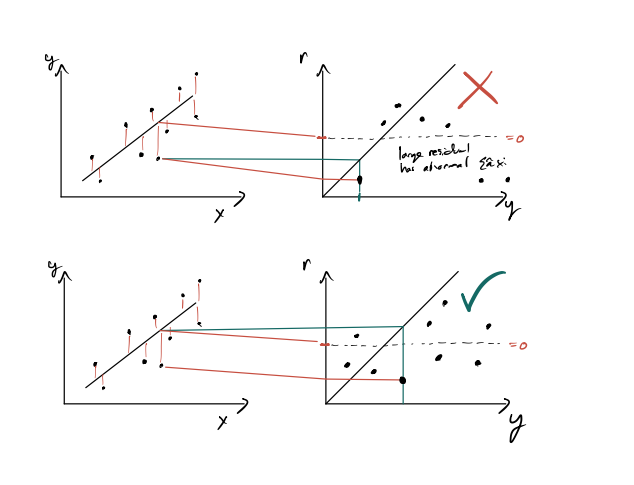
\includegraphics[width=0.8\textwidth]{./../figures/res}
%    \caption{Correct and incorrect way to plot residuals against response variable }
%    \label{fig:res}
%\end{figure}

\begin{example}[Residual plots]\label{ex:res}

Consider the regression model with two predictors and suppose the true parameter values are $\beta_0=0$,$\beta_1 = 0.2$,$\beta_2 = 20$ and $\sigma = 1$. \\


\noindent
\underline{Question:} Compare two ways of plotting the residuals 
\begin{enumerate}[label=(\alph*)]
\item Plot $r_i$ as a function of $\sum_i^{K} \hat{\beta}_iX_{i,j}$. 
\item Plot $r_i$ as a function of $Y_i$. Why does there appear to be a bias towards high values of $r_i$ for large $Y_i$ that is not present in the first plot? \\
\end{enumerate}


\noindent
\underline{Solution:} See \href{https://colab.research.google.com/drive/1q3mfX4od6iLFHy2dYFaKzw6FjaTbAaD3?usp=sharing}{colab notebook}

\end{example}

\item Let's take a closer look at the mathematics underlying the residual plot.
Note that 
\begin{equation}\label{eq:resapprox}
r_j \approx Y_j - \underbrace{E[Y|(X_1,\dots,X_K) = (X_{1,j},\dots,X_{K,j})] }_{\approx \hat{y}_j}
\end{equation}
where $K$ is the number of predictors. 
Thus, the distribution of $r_j$ is approximately 
\begin{equation*}
r_j \sim {\rm Normal}(0,\sigma^2). 
\end{equation*}
This tells us how the points should be distributed in the vertical direction. It {\bf does not} say anything about the distribution of points in the horizontal direction, which is determined by the distribution of the predictors. Therefore, we expect a plot which is symmetric around the line $r_j$ for all values of $\hat{y}_j$ (our predicted values of $Y$), but any distribution in the horizontal direction is okay. 

Now compare this to what would happen if we plotted $Y_j$ on the horizontal axis, not $\hat{y}_j$. In this case, based on Equation \ref{eq:resapprox} $r_j$ and $Y_j$ are correlated. This is why we see a bias of the residuals for small/large $Y_j$ in Example \ref{ex:res}. 

\end{itemize}




%----------------------------------------------------------------------------------------------------------------
\section{Non-linear models}

\begin{itemize}
\item Here, we discuss how to build more complex models and directly access their predictive power on out-of-sample data.  %Previously, we saw that we can indirectly access it by looking at model assumptions and $R^2$
In the context of interactions, we already saw saw how a model can be extended by defining a new predictor $X_3 = X_1X_2$. The more general idea that we can define a new predictor which is a function of the other predictors allows us to develop very complex and flexible models which nonetheless can be analyzed within linear regression framework. Here, we will formalize this, beginning with the case of a single predictor. 

In general, the linear regression framework allows us to fit models of the form consider the model
\begin{equation}\label{eq:nlgauss}
Y|X \sim {\rm Normal}( f(X),\sigma^2)
\end{equation}
provided we can express $f(X)$ as a linear combinations of nonlinear functions of $X$. What I mean by this is that we can find function $\phi_1(x),\dots,\phi_K(x)$ such that 
\begin{equation*}
f(X) = \sum_{i=1}^K \beta_i\phi_i(X)
\end{equation*}
The functions $\phi_i(X)$ are often referred to as \dfn{basis functions}, or \dfn{features} in machine learning lingo. We can think of each $\phi_i(X)$ as a new predictor. 



\begin{example}[Simulating a nonlinear model]

Consider the conditional Gaussian model given in Equation \ref{eq:nlgauss} with 
\begin{equation*}
f(x) = \beta_0+\beta_1x + \beta_2x^2
\end{equation*}
 This is simply a linear model once we define the new predictors 
\begin{align*}
X_1 &= \phi_1(X) = X\\
X_2 &= \phi_2(X) = X^2. 
\end{align*}


\noindent
\underline{Question:}
\begin{enumerate}[label=(\alph*)]
\item Generate data from this model
\item Fit the data to the model using \verb!statsmodels!.\\
\end{enumerate}

\noindent
\underline{Solution:}
See \href{https://colab.research.google.com/drive/1q3mfX4od6iLFHy2dYFaKzw6FjaTbAaD3?usp=sharing}{colab notebook}

\end{example}



\begin{figure}[h]
    \centering
    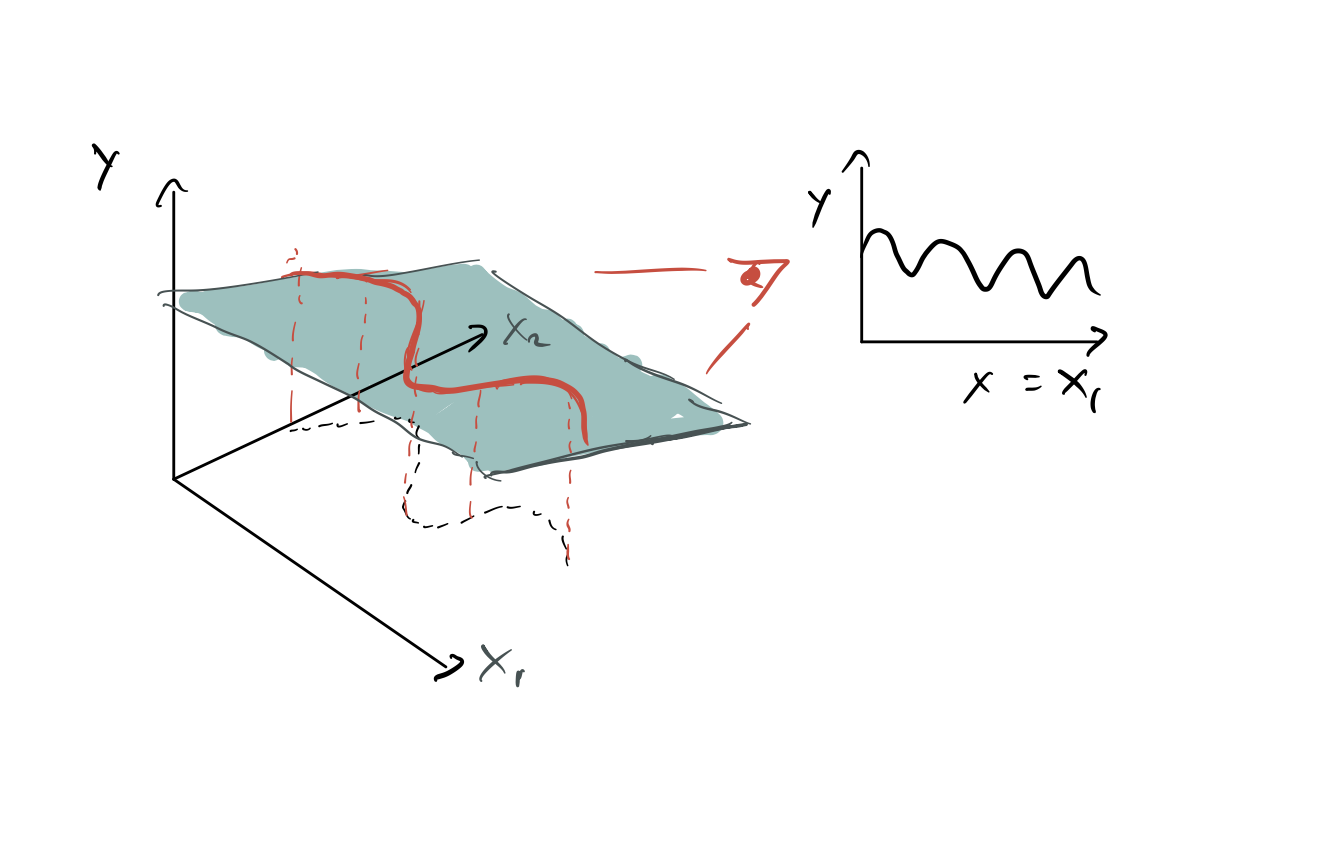
\includegraphics[width=0.8\textwidth]{./../figures/feature}
    \caption{An illustration of how a nonlinear dependence on our predictor can be incorporated into the linear modeling framework by adding a feature.}
    \label{fig:feature}
\end{figure}

\item Which functions $\phi$ should we use? The answer of course depends on the problem at hand. For example, we might know something about the physics of the data we are modeling. In some cases, we may select the $\phi$ so that the parameters $a_i$ have clear interpretations (as is the case in linear regression model). The following illustrates such an example.  

\begin{example}[Mauna Kea Data]

\noindent
\underline{Solution:} See \href{https://colab.research.google.com/drive/1q3mfX4od6iLFHy2dYFaKzw6FjaTbAaD3?usp=sharing}{colab notebook}


\end{example}

\item We now understand that within the linear regression framework we can fit very complicated nonlinear data. However, we need to be careful when adding new features to the model. The following example will illustrate how it is possible to ``overshoot'' and make our too complex. In the next set of notes we will dive much deeper into this, bridging the gap between machine learning and statistics. 
\begin{example}[Models with very large numbers of parameters]\label{ex:poly}
Consider the model 
\begin{align*}
 Y|X &\sim {\rm Normal}(f(X),\sigma^2)\\
 f(X) &= 1-X^2 + 0.9X^3
\end{align*}
This is a linear regression model with the features $X_1 = X^2$ and $X_2 = X^3$. 
We will pretend we have some data from this model, but not only do we lack knowledge of the coefficients, we in-fact lack knowledge of what the function $f(X)$ is. This, we are going to fit the data to a polynomial regression model
\begin{equation*}
f(X) = \beta_0 + \beta_1X + \beta_2X^2 + \cdots + \beta_KX^K
\end{equation*}
The question is which value of $K$ to select, since we don't know a-priori that $K=3$.  \\

\noindent
\underline{Question:} How does the predicted function $f(x)$, which we will denote $\hat{f}(x)$ compare to the true function? How does this depend on the number of features we include in our model? 
\end{example}
\end{itemize}






 \bibliographystyle{unsrt}
\bibliography{./../refs.bib}




\end{document}
